%%%%%%%%%%%%%%%%%%%%%%%%%%%%%%%%%%%%%%%%%
% University Assignment Title Page 
% LaTeX Template
% Version 1.0 (27/12/12)
%
% This template has been downloaded from:
% http://www.LaTeXTemplates.com
%
% Original author:
% WikiBooks (http://en.wikibooks.org/wiki/LaTeX/Title_Creation)
%
% License:
% CC BY-NC-SA 3.0 (http://creativecommons.org/licenses/by-nc-sa/3.0/)
% 
% Instructions for using this template:
% This title page is capable of being compiled as is. This is not useful for 
% including it in another document. To do this, you have two options: 
%
% 1) Copy/paste everything between \begin{document} and \end{document} 
% starting at \begin{titlepage} and paste this into another LaTeX file where you 
% want your title page.
% OR
% 2) Remove everything outside the \begin{titlepage} and \end{titlepage} and 
% move this file to the same directory as the LaTeX file you wish to add it to. 
% Then add \input{./title_page_1.tex} to your LaTeX file where you want your
% title page.
%
%%%%%%%%%%%%%%%%%%%%%%%%%%%%%%%%%%%%%%%%%
%\title{Title page with logo}
%----------------------------------------------------------------------------------------
%	PACKAGES AND OTHER DOCUMENT CONFIGURATIONS
%----------------------------------------------------------------------------------------

\documentclass[11pt]{article}
\usepackage[italian]{babel}
\usepackage[utf8x]{inputenc}
\usepackage{amsmath}
\usepackage{graphicx}
\usepackage[colorinlistoftodos]{todonotes}
\usepackage{enumitem}
\usepackage{listings}
\usepackage{filecontents}
\usepackage{verbatim}
\usepackage{eurosym}
\usepackage[export]{adjustbox}

\usepackage{listings}
\usepackage{xcolor}

\definecolor{codegreen}{rgb}{0,0.6,0}
\definecolor{codegray}{rgb}{0.5,0.5,0.5}
\definecolor{codepurple}{rgb}{0.58,0,0.82}
\definecolor{backcolour}{rgb}{0.95,0.95,0.92}

\lstdefinestyle{mystyle}{
    backgroundcolor=\color{backcolour},   
    commentstyle=\color{codegreen},
    keywordstyle=\color{magenta},
    numberstyle=\tiny\color{codegray},
    stringstyle=\color{codepurple},
    basicstyle=\ttfamily\footnotesize,
    breakatwhitespace=false,         
    breaklines=true,                 
    captionpos=b,                    
    keepspaces=true,                 
    numbers=left,                    
    numbersep=5pt,                  
    showspaces=false,                
    showstringspaces=false,
    showtabs=false,                  
    tabsize=2
}

\lstset{style=mystyle}

\begin{document}
\begin{titlepage}

\newcommand{\HRule}{\rule{\linewidth}{0.5mm}} % Defines a new command for the horizontal lines, change thickness here

\center % Center everything on the page
 
%----------------------------------------------------------------------------------------
%	HEADING SECTIONS
%----------------------------------------------------------------------------------------

\textsc{\LARGE Università di Messina}\\[1.5cm] % Name of your university/college
\textsc{\Large Dipartimento di scienze matematiche e informatiche, scienze fisiche e della terra}\\[0.5cm] % Major heading such as course name
\textsc{\large Corso di Laurea Triennale in Informatica}\\[0.5cm] % Minor heading such as course title

%----------------------------------------------------------------------------------------
%	TITLE SECTION
%----------------------------------------------------------------------------------------

\HRule \\[0.4cm]
{ \huge \bfseries Analisi del raffronto tra Neo4j e MongoDB nel caso di studio dell’identificazione di attività criminali}\\[0.4cm] % Title of your document
\HRule \\[1.5cm]
 
%----------------------------------------------------------------------------------------
%	AUTHOR SECTION
%----------------------------------------------------------------------------------------

\begin{minipage}{0.4\textwidth}
\begin{flushleft} \large
\emph{Autori:}\\
Gabriele \textsc{Aloisio} \textit{(503264)} \\
Samuel Giacomo \textsc{Raffa} \textit{(518206)} \\
\end{flushleft}
\end{minipage}
~
\begin{minipage}{0.4\textwidth}
\begin{flushright} \large
\emph{Docenti:} \\
prof. Antonio \textsc{Celesti} \\
prof. Massimo \textsc{Villari} \\
\end{flushright}
\end{minipage}\\[2cm]

% If you don't want a supervisor, uncomment the two lines below and remove the section above
%\Large \emph{Author:}\\
%John \textsc{Smith}\\[3cm] % Your name

%----------------------------------------------------------------------------------------
%	DATE SECTION
%----------------------------------------------------------------------------------------

{\large \today}\\[2cm] % Date, change the \today to a set date if you want to be precise

%----------------------------------------------------------------------------------------
%	LOGO SECTION
%----------------------------------------------------------------------------------------


\includegraphics[width=70px, keepaspectratio]{unime.png}\\[1cm] % Include a department/university logo - this will require the graphicx package
 
%----------------------------------------------------------------------------------------

\vfill % Fill the rest of the page with whitespace

\end{titlepage}

\tableofcontents
\pagebreak

\section{Abstract}
\pagebreak

\section{Introduzione}
In questa trattazione scientifica si descrivono le differenze del rendimento 
di calcolo tra due popolari \textit{Database Management Systems} (DBMS) di tipo NoSQL. 
I DBMS in questione sono il graph-oriented Neo4j e il document-oriented MongoDB. 
I DBMS NoSQL concedono di gestire il dato in modo più flessibile, 
rispetto al tradizionale e rigido modello tabulare dei database relazionali. 
I NoSQL infatti permettono di modellare la struttura in base alla necessità,
introducendo paradigmi strutturali come \textit{grafo, column-based e key-value},
ognuno aventi i suoi punti forti e casi obiettivo. Con essi comparirono
anche il concetto di scalabilità delle basi di dati come sistemi distribuiti,
dando vita al \textit{Teorema CAP}, di Eric Brewer. Questo teorema afferma che
\textbf{per un sistema informatico distribuito è impossibile fornire simultaneamente
tutte e tre le seguenti garanzie:}
\begin{itemize}
    \item Coerenza (copy-\textbf{c}onsistency)
    \item Disponibilità (\textbf{a}vailability)
    \item Tolleranza di partizione (\textbf{p}artitioning)
\end{itemize}
Di fatto, le uniche coppie formabili con sistemi reali sono CP, AP e CA. \\\\
In questo trattato sono illustrate le misurazioni di performance 
(tempo di esecuzione e di risposta) dei DBMS NoSQL presi in considerazione 
in riferimento a quattro query scelte con complessità computazionale incrementale.
Per questa analisi è stato scelto il caso di studio \textit{How to use graph 
technology to identify criminal activities in call records?}\cite{linkurious} presentato da Linkurious.
I test sono stati eseguiti su una macchina virtuale \textit{Debian Bullseye 11.5.0 }con 6GB di memoria RAM
e 4 core di un \textit{AMD Ryzen 7 3700X} dedicati. 
Viene utilizzato il linguaggio \textit{Python} per la generazione del dataset fittizio
e il plotting delle misurazioni tramite la libreria \texttt{matplotlib}.

\pagebreak
\section{Caso di studio}
Si pone il problema dell'identificazione dell'attività criminale tramite l'analisi
delle chiamate telefoniche effettuate nell'arco di tempo e nel luogo più inerenti al caso.
Vengono utilizzati i DBMS NoSQL per facilitare il processo di rintracciamento di soggetti o
per lo meno il restringimento del campo di ricerca. Questo viene fatto avvantaggiandosi delle rappresentazioni
di strutture dati dei DBMS NoSQL rispetto alla tradizionale rappresentazione tabulare dei DBMS classici.

Prendiamo come esempio un gruppo di criminali che compie un furto. Sappiamo che il furto è avvenuto
in un luogo $L$ ad un tempo $t$. Tramite i strumenti a nostra disposizione, possiamo
effettuare una ricerca sul database delle chiamate effettuate nel luogo $L$ ed in un intorno definito di $t$ e
grazie alla modellazione a grafo è possibile visualizzare le chiamate incrociate, permettendoci di
identificare terzi che sono inclusi indirettamente nel crimine. 

Supposto che i gestori telefonici diano accesso al database e alla sua architettura, possiamo ammettere
una struttura del tipo:

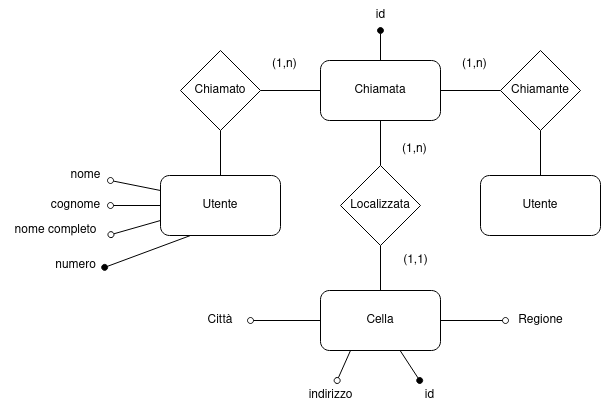
\includegraphics[width=350px, keepaspectratio]{er.png}\\[1cm]

\pagebreak
Da qui desumiamo le seguenti entità:
\begin{itemize}
    \item Utente - identificato da un \textit{numero} di telefono univoco, \textit{nome}, \textit{cognome} e \textit{nome completo}
    \item Chiamata - identificata da un \textit{id}
    \item Cella - identificata da un \textit{id,} caratterizzata da una \textit{città, indirizzo} e una \textit{regione} 
\end{itemize}

e le relazioni \textit{localizzata, Chiamante} e \textit{Chiamato}.

\section{Architettura}

    \subsection{Neo4j}
    Neo4j è un DBMS NoSQL \textit{graph-oriented} open source sviluppato in Java.
    Permette un utilizzo in modalità server ed una modalità embedded.
    Lanciato in modalità server il database è un processo indipendente a cui
    si accede tramite lo stile architetturale REST. Sono supportati i plugin. 
    In modalità embedded, il processo incorpora il database nell'applicazione 
    Java e viene eseguito all'interno della JVM. Per l'importazione massiva di dati 
    è supportata l'esecuzione in modalità non concorrente. Al dato importato 
    è possibile crearne un nodo ed assegnarvi il tipo di dato (tipi elementari 
    di Java) ed un nome. Come risultato abbiamo un grafo \textit{schema-less}, che Permette 
    un'eterogeneità del dato con il minimo sforzo. Neo4j si mostra
    molto efficiente nell'estrazione e rappresentazione di strutture
    ad albero come nei file XML, filesystem e reti. Da questo derivano
    implementazioni pronte all'uso di operazioni più comuni sui grafi
    come l'algoritmo di Dijkstra e ricerca dei cicli. Risulta invece scomodo
    nelle ricerche complesse, per esempio basate su confronti matematici e non
    supporta lo \textit{sharding.}

    \subsection{MongoDB}
    MongoDB è un DBMS NoSQL \textit{document-oriented.} Si basa sulla memorizzazione
    in base di documenti in formato \textit{BSON,} ispirato al JSON ma con l'aggiunta
    della dinamicità. Supporta query \textit{ad hoc} per la ricerca su base
    \textit{regex}, intervalli o campi. Qualsiasi campo è indicizzabile, anche
    con indici secondari, unici, sparsi, geospaziali e full-text. MongoDB dispone
    dei textit{replica set,} cioè due o più copie di dati. Ogni copia è identificata come
    primaria o secondaria. Quando una replica primaria fallisce viene avviato un processo
    per la determinazione della copia più adatta a sostituire quella primaria. Lo sharding
    permette a MongoDB di scalare orizzontalmente, implementanto inoltre un
    meccanismo di load-balancing. La funzione GridFS permette di utilizzare il DBMS come file system,
    esponendo agli sviluppatori delle funzioni per la manipolazione del dato. GridFS divide il file
    in chunks e memorizza ognuno di questi in un documento separato.  

    \subsection{Python}
    Python è un linguaggio di programmazione orientato agli oggetti. Si è scelto di utilizzare questo
    linguaggio per la semplicità di utilizzo e la facile disponibilità dei driver per accedere e manipolare
    i database MongoDB e Neo4j. In questo caso si utilizza la libreria \textit{Faker} per generare i dati fittizi.

\section{Implementazione}
    Come visto nella sezione 3, abbiamo esumato delle entità e relazioni. Queste sono state implementate
    nei due DMBS nel loro rispettivo modo.

    \subsection{Neo4j}

    Sono definiti i seguenti nodi
    \begin{itemize}
        \item \textit{cell}:
            \begin{itemize}
                \item cell\_site, ID
                \item state
                \item city
                \item address
            \end{itemize}

        \item \textit{person}:
            \begin{itemize}
                \item first\_name
                \item last\_name
                \item full\_name
                \item number
            \end{itemize}

        \item \textit{call}:
            \begin{itemize}
                \item calling\_number
                \item called\_number
                \item start\_date
                \item end\_date
                \item duration
                \item cell\_cite, si riferisce al cell\_site di \textit{cell}
            \end{itemize}
    \end{itemize}

    E i seguenti archi (\textit{label})

    \begin{itemize}
        \item \textit{made\_call}: person.number $\rightarrow$ call.calling\_number
        \item \textit{received\_call}: call.called\_number $\rightarrow$ person.number
        \item \textit{located\_in}: call.cell\_site $\rightarrow$ cell.cell\_site
    \end{itemize}



    \subsection{MongoDB}
    Sono definite le seguenti collezioni
    \begin{itemize}
        \item \textit{cells}:
            \begin{itemize}
                \item cell\_site, ID
                \item state
                \item city
                \item address
            \end{itemize}

        \item \textit{people}:
            \begin{itemize}
                \item first\_name
                \item last\_name
                \item full\_name
                \item number
            \end{itemize}

        \item \textit{calls}:
            \begin{itemize}
                \item calling\_number
                \item called\_number
                \item start\_date
                \item end\_date
                \item duration
                \item cell\_cite, si riferisce al cell\_site di \textit{cell}
            \end{itemize}
    \end{itemize}

    E le relazioni
    \begin{itemize}
        \item \textit{made\_call}: person.number $\rightarrow$ call.calling\_number
        \item \textit{received\_call}: call.called\_number $\rightarrow$ person.number
        \item \textit{located\_in}: call.cell\_site $\rightarrow$ cell.cell\_site
    \end{itemize}

    \subsection{Generazione dei dati}
    Si generano quattro dataset di dimensioni diverse da inserire successivamente sui database
    MongoDB e Neo4j. Le dimensioni stabilite sono 100\%, 75\%, 50\%, 25\%, che indicano rispettivamente
    le dimensioni dei dataset in base al dataset con il 100\% del contenuto di informazioni.
    Per popolare il database con dati fittizi, si è scritto un codice Python che utilizza Faker.
    Il file \texttt{config.ini} contiene i parametri fissi che indicano il numero di record da generare.
    Al momento dell'avvio dello script viene passato un parametro $L$ che indica la percentuale
    del carico in base a questi valori. 
    Come valori predefiniti si è scelto 50000 persone, 10000 celle e 200000 chiamate.
    
    \begin{lstlisting}[caption=config.ini]
[load]
MAX_PEOPLE=50000
MAX_CELLS=10000
MAX_CALLS=200000
    \end{lstlisting}

    \pagebreak
    Il file \texttt{datasetgen.py} si occupa della generazione dei dati.
    È definita una funzione per ogni entità:
    
    \begin{lstlisting}[language=Python, caption=gen\_people()]
def gen_people(size: int):
    with open(data_path("people.csv"), 'w', newline='') as file:
        writer = csv.writer(file)
        writer.writerow(['first_name', 'last_name', 'full_name', 'number'])

        for i in range(size):
            name = fake.name().split()

            #genera un numero univoco (simulazione di un do-while)
            while True:
                number = gen_fake_phone_number()
                if number not in people:
                    break

            writer.writerow([name[0], name[1], " ".join(name), number])
            people.append(number)

        file.close()
    \end{lstlisting}

    \begin{lstlisting}[language=Python, caption=gen\_cells()]
def gen_cells(size: int):
    global ncells

    with open(data_path("cells.csv"), 'w', newline='') as file:
        writer = csv.writer(file)
        writer.writerow(['cell_site', 'city', 'address', 'state'])

        for i in range(size):
            city = fake.city()
            address = fake.street_name()
            state = fake.current_country_code()

            writer.writerow([i, city, address, state])

        file.close()
    
    \end{lstlisting}

    \pagebreak
    \begin{lstlisting}[language=Python, caption=gen\_calls()]
def gen_calls(size: int):
    npeople = len(people)

    with open(data_path("calls.csv"), 'w', newline='') as file:
        writer = csv.writer(file)
        writer.writerow(['calling_number', 'called_number', 'start_date', 'end_date', 'duration', 'cell_site'])

        for i in range(size):
            caller = randint(0, npeople-1)

            #prende ripetutamente un numero dalla lista delle persone se il numero del chiamante e' uguale a quello del chiamato
            while True:
                called = randint(0, npeople-1)
                if called != caller:
                    break

            duration = randint(0, 1000)
            cell_site = randint(0, ncells-1)

            #data di inizio [solo anno attuale]
            start_date = fake.date_time_this_year()

            #la data di fine della chiamata equivale alla data di inizio della chiamata + la durata(in secondi)
            end_date = start_date + timedelta(seconds=duration)

            writer.writerow([people[caller], people[called], int(round(datetime.timestamp(start_date))), int(round(datetime.timestamp(end_date))), duration, cell_site])
        file.close()
    
    \end{lstlisting}

    \pagebreak
    \subsection{Importazione dei dati}
    I record vengono letti dai file \texttt{csv} esportati in precedenza. Tramite
    la funzione \texttt{load\_data()} in \texttt{mongo\_manager.py} 
    è possibile caricare i dati su MongoDB, mentre Neo4j importa automaticamente i file \texttt{csv}
    che sono presenti nella directory \texttt{/relate-data/dbmss/<database id>/import} di Neo4j.
    \\ 

    \begin{lstlisting}[language=Python, caption=load\_data()]
def load_data(handle: MongoClient):
db = handle.progettodb2

with open(data_path('cells.csv'), "r") as cfile:
    db.cells.insert_many(to_dict(list(DictReader(cfile))))

    cfile.close()

with open(data_path('people.csv'), "r") as pfile:
    db.people.create_index("number", unique=True)
    db.people.insert_many(to_dict(list(DictReader(pfile))))

    pfile.close()

with open(data_path('calls.csv'), "r") as cafile:
    db.calls.insert_many(to_dict(list(DictReader(cafile))))

    cafile.close()
        
    \end{lstlisting}


\pagebreak
\section{Risultati degli esperimenti}
Le query presentate di seguito sono definite nei file sorgenti \texttt{mongo\_queries.py} e 
\texttt{neo\_queries.py}. I valori \texttt{gt\_start} e \texttt{lt\_start} definiscono
rispettivamente la data massima e la data minima (in formato \textit{epoch}) delle chiamate da prendere
in considerazione. Il valore \texttt{duration} definisce la durata massima delle chiamate.
\\
È stato utilizzato LibreOffice Calc per la manipolazione dei dati e
la generazione dei grafici a seguire.

    \subsection{2 WHERE}
    Viene effettuata una selezione condizionata con due clausole \texttt{WHERE}

    \begin{lstlisting}[language=Python, caption=Neo4j]
"MATCH (c:call) WHERE c.start_date >" 
+ str(gt_start) 
+ " AND c.start_date < " 
+ str(lt_start) 
+ " RETURN c"
    \end{lstlisting}

    \begin{lstlisting}[language=Python, caption=MongoDB]
{
    "$match": {
        "start_date": {
            "$gte": gt_start,
            "$lt": lt_start
        }
    }
}
    \end{lstlisting}

    \begin{figure}
        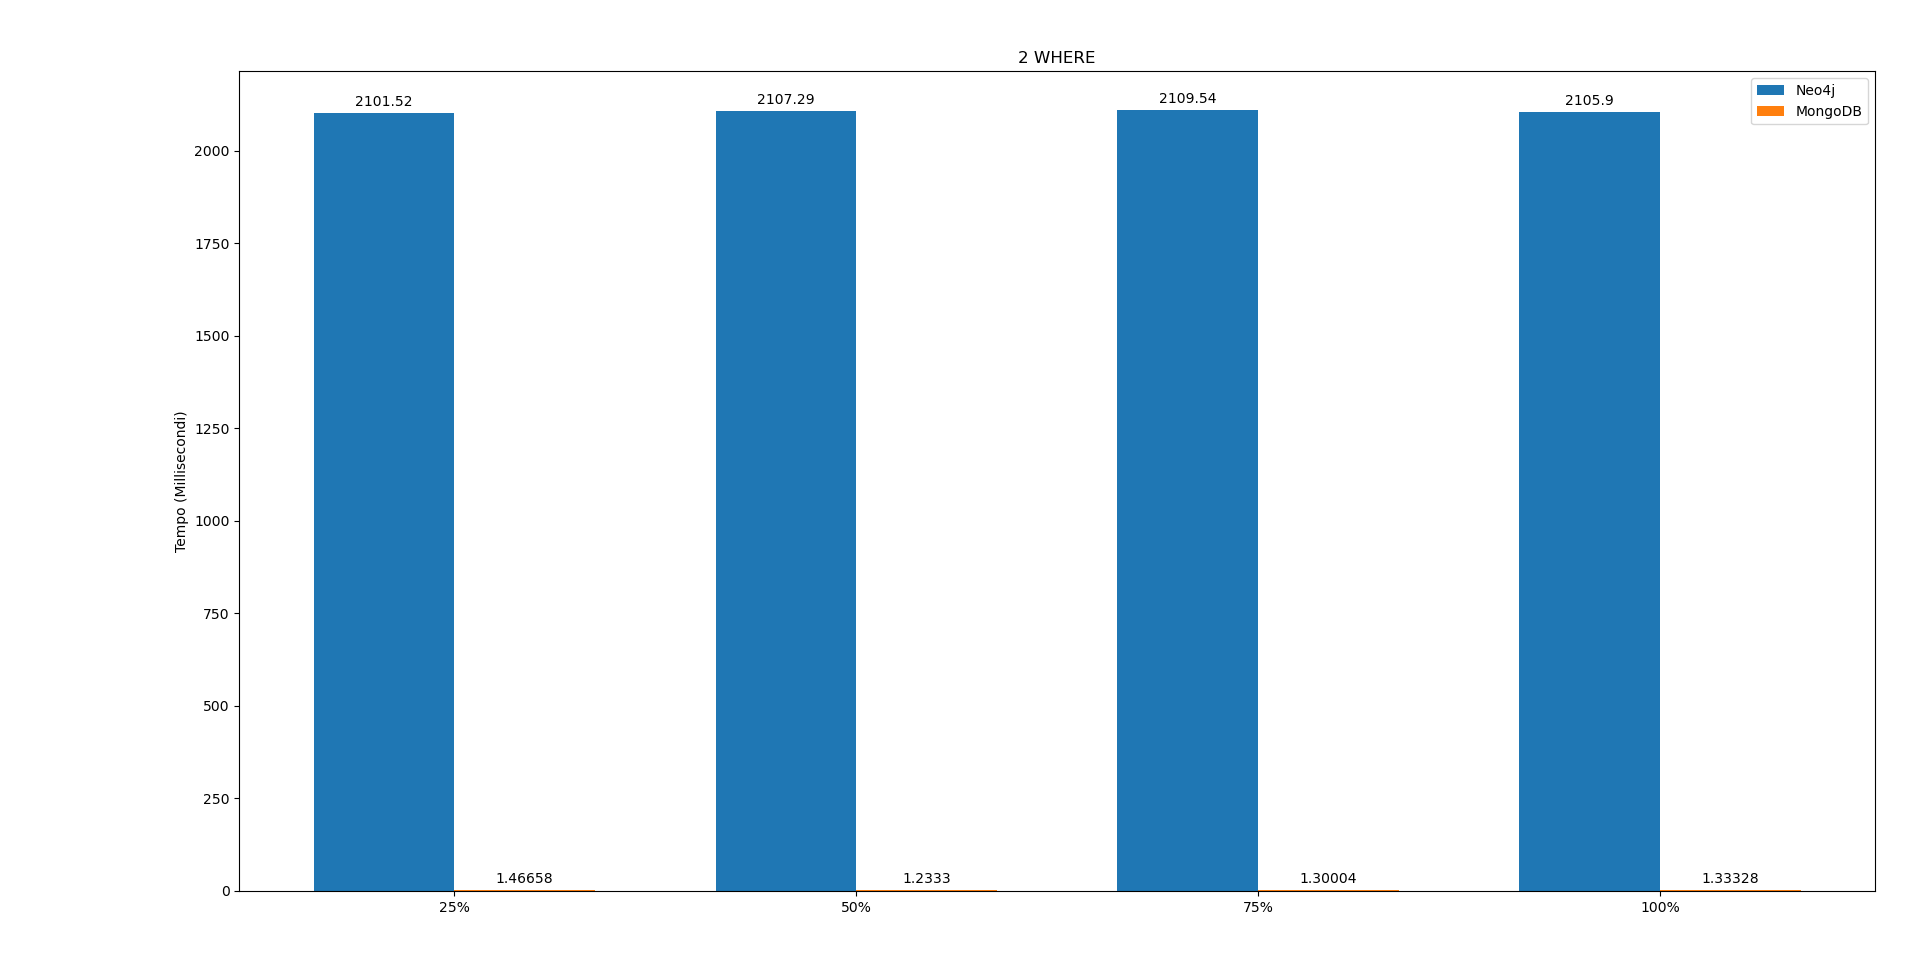
\includegraphics[width=320px, keepaspectratio, center]{query1.png}
        \label{fig:results1}
        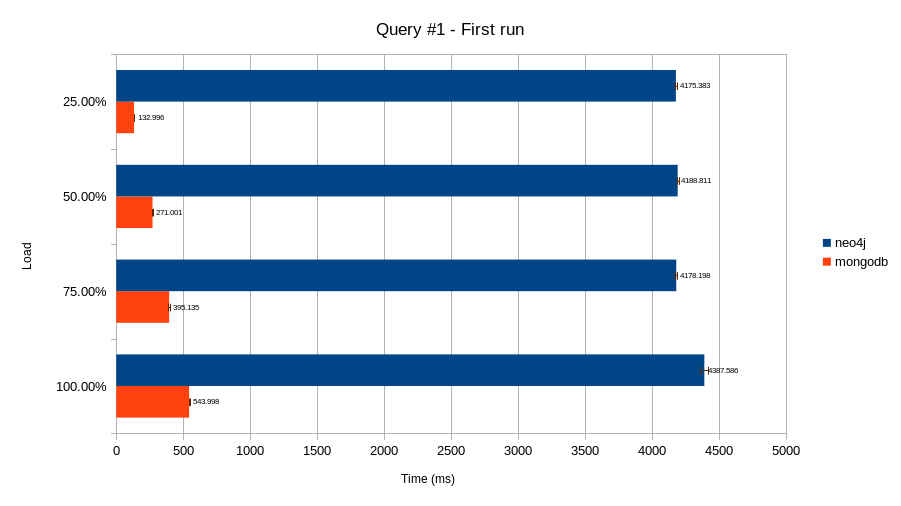
\includegraphics[width=350px, keepaspectratio, center]{query1_fr.png}
        \label{fig:query1_fr}
        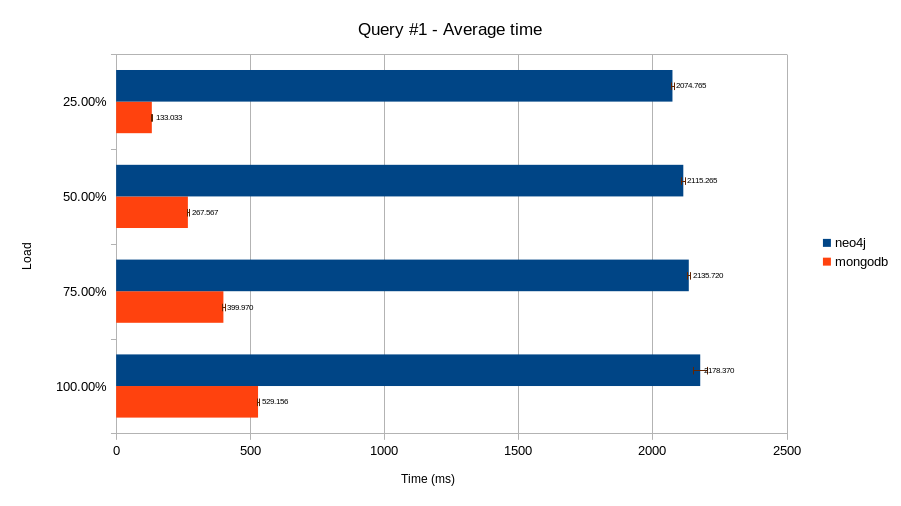
\includegraphics[width=350px, keepaspectratio, center]{query1_avg.png}
        \label{fig:query1_avg}
    \end{figure}    


\pagebreak
    \subsection{3 WHERE}
    Viene effettuata una selezione condizionata con tre clausole \texttt{WHERE}
    e un \texttt{JOIN}

    \begin{lstlisting}[language=Python, caption=Neo4j]
"MATCH (c:call) WHERE c.start_date > " 
+ str(gt_start) 
+ " AND c.start_date < " 
+ str(lt_start) 
+ " AND c.duration >= " 
+ str(duration) 
+ " RETURN c"

    \end{lstlisting}


    \begin{lstlisting}[language=Python, caption=MongoDB]
{
    "$match": {
        "start_date": {
            "$gte": gt_start,
            "$lt": lt_start
        },
        "duration": {
            "$gte": duration
        }
    }
}
    \end{lstlisting}
    
    \begin{figure}
        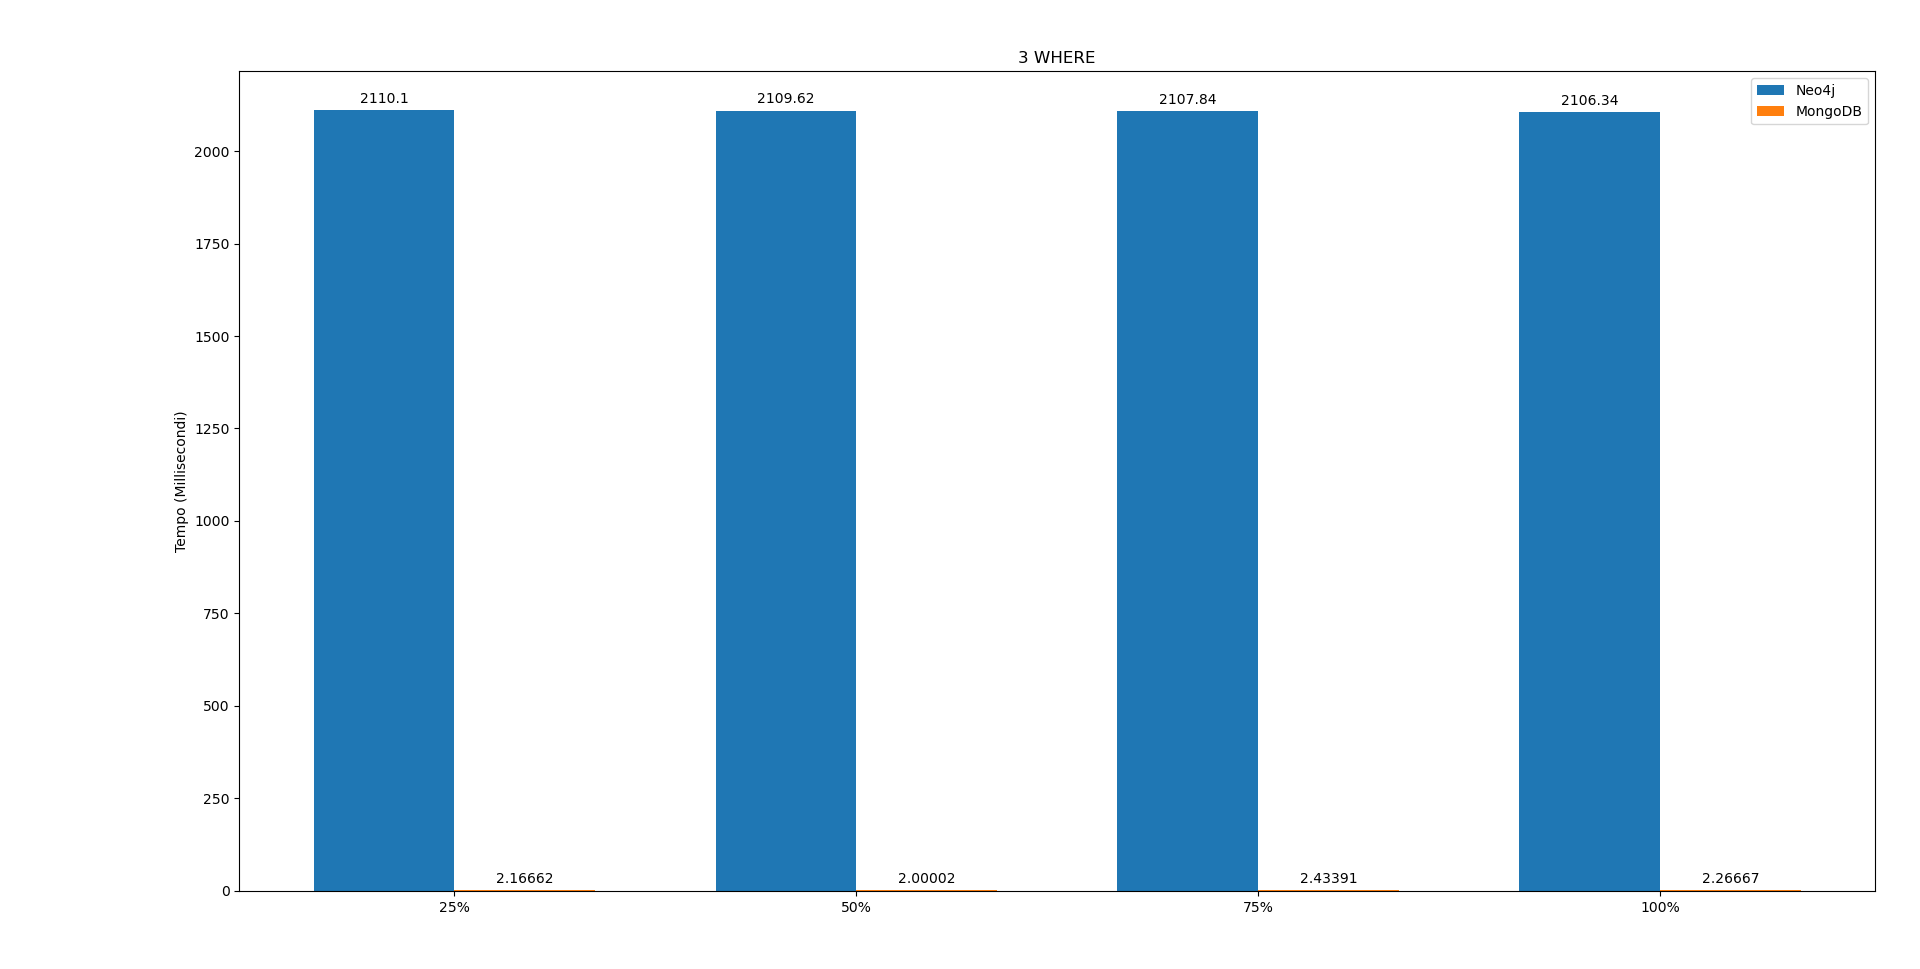
\includegraphics[width=320px, keepaspectratio, center]{query2.png}
    \label{fig:results2}
        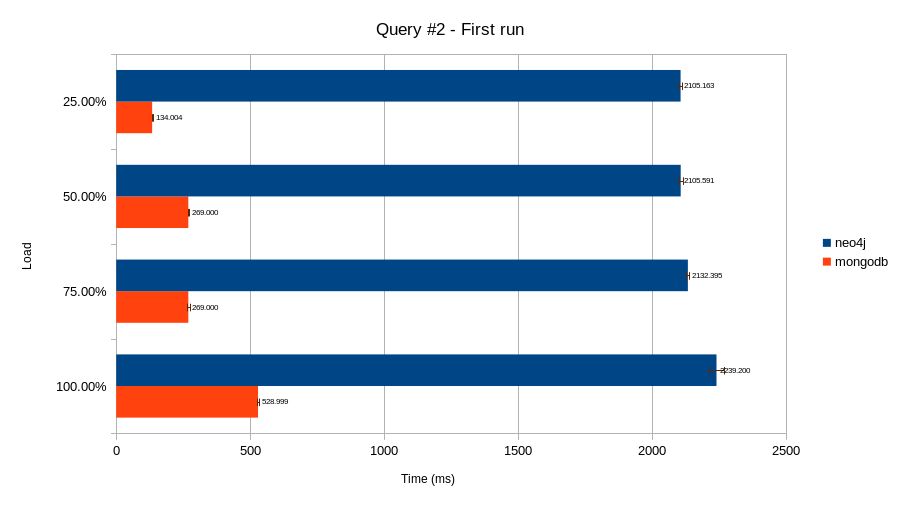
\includegraphics[width=350px, keepaspectratio, center]{query2_fr.png}
        \label{fig:query2_fr}
        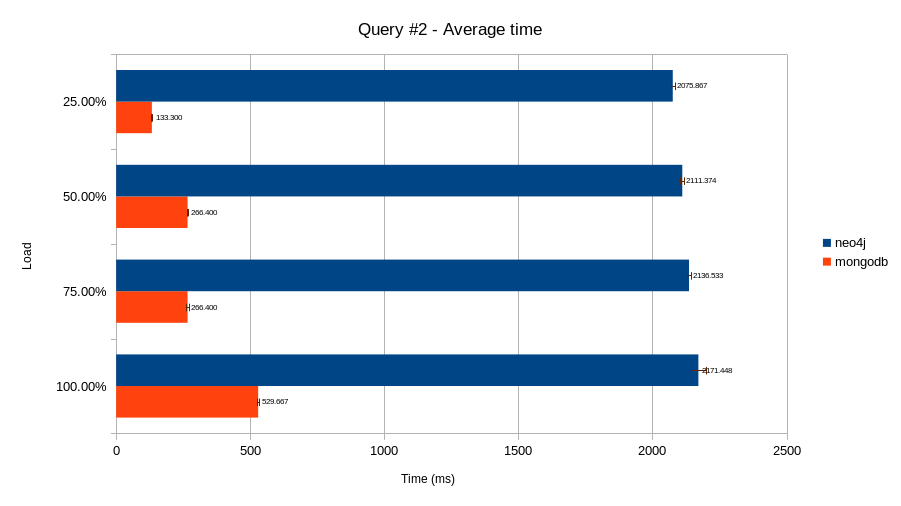
\includegraphics[width=350px, keepaspectratio, center]{query2_avg.png}
        \label{fig:query2_avg}
    \end{figure}

    \pagebreak
    \subsection{3 WHERE 1 JOIN}
    Viene effettuata una selezione condizionata con tre clausole \texttt{WHERE}
    e un \texttt{JOIN}

    \begin{lstlisting}[language=Python, caption=Neo4j]
"MATCH (p:person)-[r:made_call]->(c:call) WHERE c.start_date >" 
+ str(gt_start) 
+ " AND c.start_date < " 
+ str(lt_start) 
+ " AND c.duration >= " 
+ str(duration) 
+ " RETURN c, r, p"
    \end{lstlisting}


    \begin{lstlisting}[language=Python, caption=MongoDB]
{
    "$match": {
        "start_date": {
            "$gte": gt_start,
            "$lt": lt_start
        },
        "duration": {
            "$gte": duration
        }
    }
},
{
    "$lookup": {
        "from": "people",
        "localField": "calling_number",
        "foreignField": "number",
        "as": "caller"
    }
}
    \end{lstlisting}

    \begin{figure}
        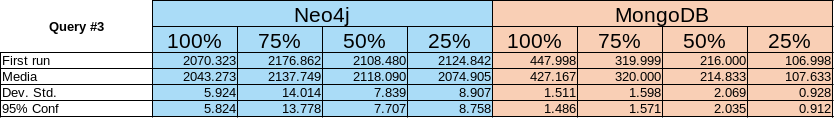
\includegraphics[width=320px, keepaspectratio, center]{query3.png}
        \label{fig:results3}
        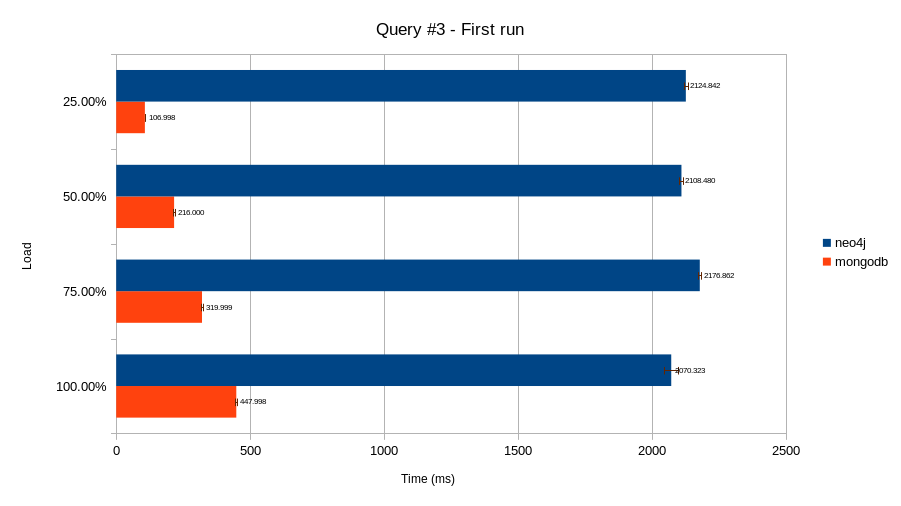
\includegraphics[width=350px, keepaspectratio, center]{query3_fr.png}
        \label{fig:query3_fr}
        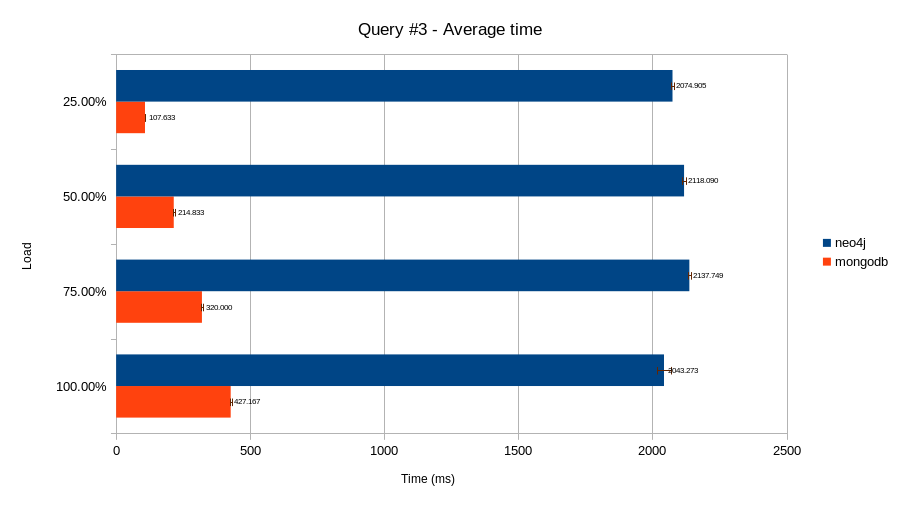
\includegraphics[width=350px, keepaspectratio, center]{query3_avg.png}
        \label{fig:query3_avg}
    \end{figure}

    \pagebreak
    \subsection{3 WHERE 2 JOIN}
    Viene effettuata una selezione condizionata con tre clausole \texttt{WHERE}
    e due \texttt{JOIN}

    \begin{lstlisting}[language=Python, caption=Neo4j]
"MATCH(p:person)-[r1:made_call]->(c:call)-[r2:located_in]->(ce:cell) WHERE c.start_date >" 
+ str(gt_start) 
+ " AND c.start_date < " 
+ str(lt_start) 
+ " AND c.duration >= " 
+ str(duration) 
+ " RETURN c,p,r1,r2,ce"
    \end{lstlisting}


    \begin{lstlisting}[language=Python, caption=MongoDB]
{
    "$match": {
        "start_date": {
            "$gte": gt_start,
            "$lt": lt_start
        },
        "duration": {
            "$gte": duration
        }
    }
},
{
    "$lookup": {
        "from": "people",
        "localField": "calling_number",
        "foreignField": "number",
        "as": "caller"
    }
},
{
    "$lookup": {
        "from": "cells",
        "localField": "cell_site",
        "foreignField": "cell_site",
        "as": "cell"
    }
}
    \end{lstlisting}

    \begin{figure}
        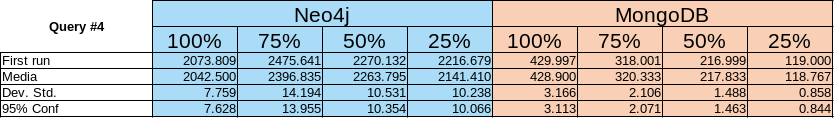
\includegraphics[width=320px, keepaspectratio, center]{query4.png}
    \label{fig:results4}
        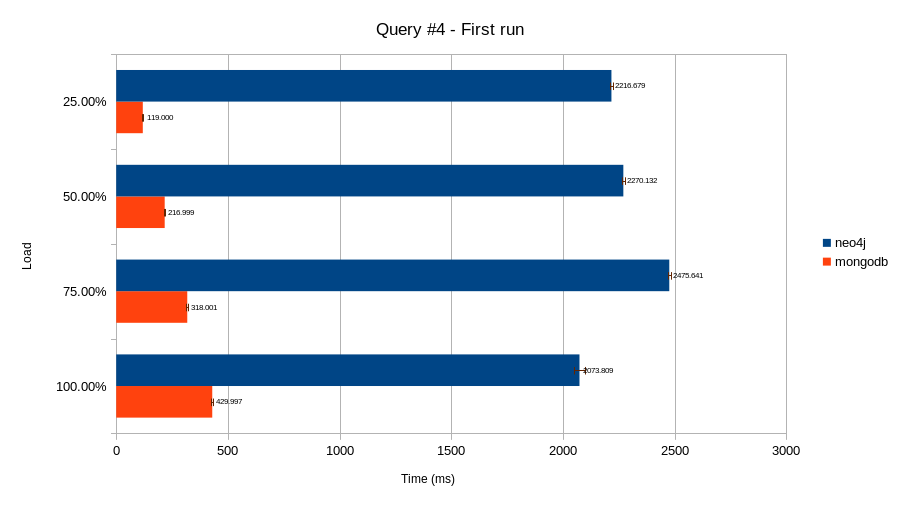
\includegraphics[width=350px, keepaspectratio, center]{query4_fr.png}
        \label{fig:query4_fr}
        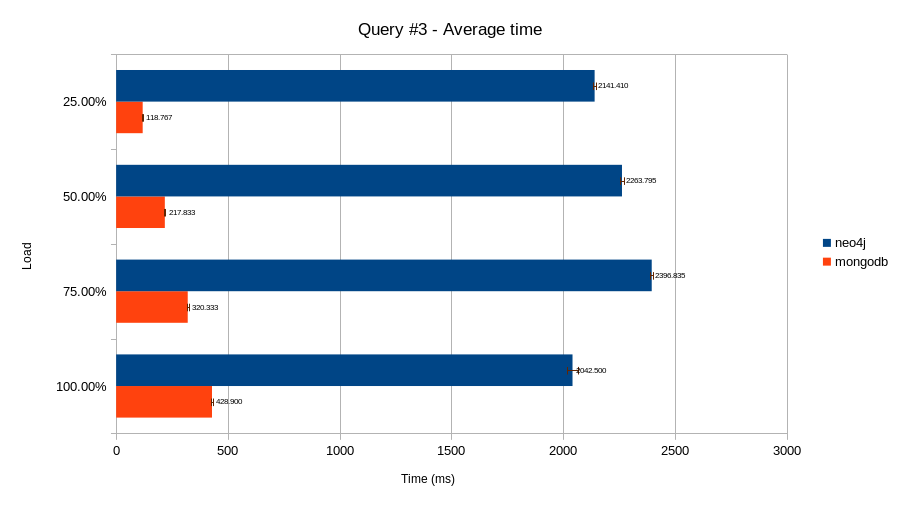
\includegraphics[width=350px, keepaspectratio, center]{query4_avg.png}
        \label{fig:query4_avg}
    \end{figure}


\section{Conclusioni}
Si osserva che MongoDB è in vantaggio consistente per dataset di medie dimensioni e che 


\begin{thebibliography}{1}
\bibitem{linkurious} https://linkurious.com/blog/how-to-use-phone-calls-and-network-analysis-to-identify-criminals/
\end{thebibliography}

\end{document}